\section{【实现】显示字符串}\label{ux5b9eux73b0ux663eux793aux5b57ux7b26ux4e32}

bootloader只在CPU和内存中打转无法让读者很容易知道bootloader的工作是否正常,为此在成功完成了保护模式的转换后,就需要通过显示字符串来展示一下自己了。bootloader设置好栈后,就可以调用bootmain函数显示字符串了。在proj1中使用了显示器和并口两种外设来显示字符串,主要的代码集中在bootmain.c中。

这里采用的是很简单的基于Programmed I/O
(PIO)方式,PIO方式是一种通过CPU执行I/O端口指令来进行数据读写的数据交换模式,被广泛应用于硬盘、光驱等设备的基础传输模式中。这种I/O访问方式使用CPU
I/O端口指令来传送所有的命令、状态和数据,需要CPU全程参与,效率较低,但编程很简单。后面讲到的中断方式将更加高效。
在bootmain.c中的lpt\_putc函数完成了并口输出字符的工作。输出一个字符的流程(可参看bootmain.c中的lpc\_putc函数实现)大致如下:

\begin{enumerate}
\def\labelenumi{\arabic{enumi}.}
\tightlist
\item
  读I/O端口地址0x379,等待并口准备好;
\item
  向I/O端口地址0x378发出要输出的字符;
\item
  向I/O端口地址0x37A发出控制命令,让并口处理要输出的字符。
\end{enumerate}

在bootmain.c中的serial\_putc函数完成了串口输出字符的工作。输出一个字符的流程(可参看bootmain.c中的serial\_putc函数实现)大致如下:

\begin{enumerate}
\def\labelenumi{\arabic{enumi}.}
\tightlist
\item
  读I/O端口地址(0x3f8+5)获得LSR寄存器的值,等待串口输出准备好;
\item
  向I/O端口地址0x3f8发出要输出的字符;
\end{enumerate}

在bootmain.c中的cga\_putc函数完成了CGA字符方式在某位置输出字符的工作。输出一个字符的流程(可参看bootmain.c中的cga\_putc函数实现)大致如下:

\begin{enumerate}
\def\labelenumi{\arabic{enumi}.}
\tightlist
\item
  写I/O端口地址0x3d4,读I/O端口地址0x3d5,获得当前光标位置;
\item
  在光标的下一位置的显存地址空间上写字符,格式是黑色背景/白色字符;
\item
  设置当前光标位置为下一位置。
\end{enumerate}

proj1启动后的PC机内存布局如下图所示:

\begin{figure}[htbp]
\centering
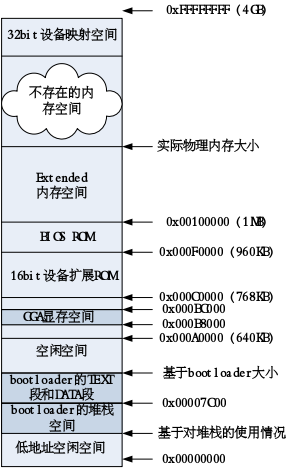
\includegraphics{figures/3.18.1.png}
\caption{3.18.1}
\end{figure}

自此,我们了解了一个小巧的bootloader的实现过程,但这还仅仅是百尺竿头的第一步,它还只能显示字符串,不能加载操作系统。我们还需要扩展bootloader的功能,让它能够加载操作系统。
